\documentclass[12pt]{report}
\usepackage{greg}
\usepackage{agda}
\usepackage[baskerville,vvarbb]{newtxmath}
\usepackage{fontspec}
\usepackage{titlesec}
\usepackage[nottoc]{tocbibind}

\setmainfont{Baskerville}
\setsansfont{Quadrat-Serial}
\setmonofont{Courier New}

\titleformat*{\section}{\large\sffamily}
\titleformat*{\subsection}{\normalsize\sffamily}
\titleformat*{\subsubsection}{\normalsize\sffamily}
\titleformat{\chapter}[hang]{\LARGE\sffamily}{\LARGE\thechapter}{1ex}{}[]
\titleformat{name=\chapter,numberless}[hang]{\LARGE\sffamily}{}{0ex}{}[]

\title{Gauge Theory in Homotopy Type Theory}
\author{Greg Langmead}

\begin{document}

\begin{titlepage}
\centering
\parbox[b]{2\textwidth}{
	\vspace{6\baselineskip}
	{\Huge\sffamily Gauge Theory in\\ Homotopy Type Theory}\\[2\baselineskip]
	{\Large\rmfamily{Greg Langmead}}

	\vspace{0.47\textheight}
	{\noindent Carnegie Mellon University}\\[0.1\baselineskip]
	{\noindent \today}\\[\baselineskip]
}
\end{titlepage}

\chapter*{Abstract}
This thesis will show how to formalize parts of differential geometry, gauge theory, and Chern-Weil theory in homotopy type theory.

\tableofcontents

\mychapter{Introduction}
Differential geometry\cite{kobayashinomizu} \cite{baez1994gauge}, gauge theory \cite{hamilton2017} \cite{atiyah1983yang}, and Chern-Weil theory\cite{freed2013chernweil} lie at the intersection of mathematics and physics. The theory of general relativity is expressed as formulas relating the curvature of spacetime to the distribution of energy and matter. The standard model of particle physics is expressed as a collection of principal bundles and associated vector bundles, sections of which represent the fields of matter and forces. And in the latter decades of the 20th century the tools of the standard model were applied back into mathematics to make discoveries about the geometry of 3- and 4-dimensional manifolds\cite{scorpan_wild_2005}.

Homotopy type theory\cite{hottbook} seems at first like it's from a different universe entirely. It grew out of questions of a foundational nature inside mathematics and computer science. It brings a synthetic stance, where we are invited to stop thinking of mathematical objects as sets with structure, and instead to assemble the objects into higher categories with collective properties like being locally cartesian closed, or having homotopical model structures. Such categories have internal languages, which are syntactic structures much like programming languages, which allow us to reason about the objects in a generic way.

\mychapter{Groups}
Group theory including the theory of higher groups is built directly into HoTT, via the identity types. A thorough introductory treatment of group theory that adopts this philosophy can be found in the book \emph{Symmetry} \cite{Symmetry}. We will build on this synthetic framework to explore gauge theory. But it's important to be clear that this is a choice, and there is an alternate approach. Namely we could define a group to be a type together with some extra structure: an identity, a multiplication operation, and an inverse operation, satisfying some properties. We would do the same for higher groups, and we'd prove an equivalence between the type of higher groups and the type of pointed, connected types. Such a project has been undertaken in the context of higher topos theory, but at the time of this writing it hasn't been done inside HoTT. We certainly can define the type of groups which are sets, and prove that this type of 0-groups is equivalent to connected 1-types, and this is done in \emph{Symmetry}. But in the case of higher groups we only have one definition: pointed connected types. This happens to be a lovely theory, and so we'll be glad to run with that.

Definition: a group is a pointed 1-type $BG$ with basepoint $*$, which is connected, i.e. that we have a term of the type $(a:BG)\to||*=a||_{-1}$. We denote the type $*=*$ by $G$, and so if we have a particular group in mind then we think of that group as being installed as the identity type of the basepoint in a type we call $BG$.

\mysection{Group actions}
Given any pointed type $X$ with basepoint $x$ we can form the type $\BAut_x(X)$ by taking the connected component of $x$. If we consider the terms of $X$ to be at type-theoretic level 0, then $\Aut_x$ brings one of the identity types from level 1 down to level 0 to look at it on its own. Then the B can be thought of as reinstalling the identity type at level 1 of the new type, which contains only the connected component of $x$. When we do this, though, we don't forget the identity types of all the other terms in the connected component. That's why there really isn't a true B operator, just a notation that is meant to evoke the classical idea of a classifying space, since as we'll see we really have captured that idea.

A homomorphism of groups is a pointed map $f:BG\to X$. The rules of type theory will ensure that this map contains a map between the identity types inside the types, forming a homomorphism in the usual sense. We can think of $G$ acting on $x$ since the homomorphism is $*=*\to x=x$. If we take $X=\uni$ to be the universe, and if $f(*)=H$, then we can think of $G$ acting on the type $H$.

\mysection{Equivariant maps}

\mychapter{Principal bundles}

\mysection{Bundles over $BG$}
Pointed connected types $BG$ come with three built-in type families by choosing identity types with different endpoints. There's $LG:=(a:BG)\times a=a$ which is at each point the group of self-identifications of that point. There's $EG:=(a:BG)\times *=a$ which aren't groups, but which are similar to the self-identifications, and in fact are torsors over $G$! At each point $a:BG$ we can concatenate a term of $EG(a)$ with a term of $LG(a)$ by concatenating the latter to the $a$ endpoint of $EG(a)$. And lastly there's the non-dependent type $BG\times G$ which I'm mentioning because we can also concatenate a term of $EG(a)$ with a term of $G$, by attaching it to the $*$ endpoint.

$EG$ is contractible (Lemma 3.11.8 of The HoTT Book\cite{hottbook}). It's worth reflecting for a moment on the fact that $EG$ is contractible but $BG$ is not. After all, $BG$ is connected and so all its terms are equal to the base point via some path. But we don't select any specific paths as part of the data. Forming $EG$ is simply to install all the solutions to this missing data as the fibers of a bundle over $BG$.

Example: for $G=\zz, \zz^n, \zz_2 $ provide $BG$, $EG$, and $LG$.

\mysection{Mapping into $BG$}
Pulling back $EG$ via a map $X\to BG$ deserves to be called a principal $G$-bundle over $X$, and pulling back $LG$ via the same map deserves to be called a gauge transformation.

In HoTT given a map $f:A\to B$ and a type family $P:B\to \uni$ we can form the following square and it will commute and be a pullback:
% https://q.uiver.app/?q=WzAsNCxbMiwwLCIoYjpCKVxcdGltZXMgUChiKVxccXVhZFxccXVhZCJdLFsyLDEsIkIiXSxbMCwwLCIoYTpBKVxcdGltZXMgUChmKGEpKSJdLFswLDEsIkEiXSxbMCwxLCJcXG1hdGhybXtwcn1fMSJdLFsyLDAsIlxcbGFtYmRhKGEsIHApLihmKGEpLHApIl0sWzMsMSwiZiIsMl0sWzIsMywiXFxtYXRocm17cHJ9XzEiLDJdXQ==
\[\begin{tikzcd}
	{(a:A)\times P(f(a))} && {(b:B)\times P(b)} \\
	A && B
	\arrow["{\mathrm{pr}_1}", from=1-3, to=2-3]
	\arrow["{\lambda(a, p).(f(a),p)}", from=1-1, to=1-3]
	\arrow["f"', from=2-1, to=2-3]
	\arrow["{\mathrm{pr}_1}"', from=1-1, to=2-1]
\end{tikzcd}\]

If we have an arbitrary type $X$ and $f:X\to BG$ then we can pull back $EG$ this way:
% https://q.uiver.app/?q=WzAsNCxbMiwwLCIoYjpCRylcXHRpbWVzICgqPWIpIl0sWzIsMSwiQkciXSxbMCwwLCIoeDpYKVxcdGltZXMgKCo9Zih4KSkiXSxbMCwxLCJYIl0sWzAsMSwiXFxtYXRocm17cHJ9XzEiXSxbMiwwLCJcXGxhbWJkYSh4LCBwKS4oZih4KSxwKSJdLFszLDEsImYiLDJdLFsyLDMsIlxcbWF0aHJte3ByfV8xIiwyXV0=
\[\begin{tikzcd}
	{(x:X)\times (*=f(x))} && {(b:BG)\times (*=b)} \\
	X && BG
	\arrow["{\mathrm{pr}_1}", from=1-3, to=2-3]
	\arrow["{\lambda(x, p).(f(x),p)}", from=1-1, to=1-3]
	\arrow["f"', from=2-1, to=2-3]
	\arrow["{\mathrm{pr}_1}"', from=1-1, to=2-1]
\end{tikzcd}\]

or we can pull back $LG$:
% https://q.uiver.app/?q=WzAsNCxbMiwwLCIoYjpCRylcXHRpbWVzIChiPWIpIl0sWzIsMSwiQkciXSxbMCwwLCIoeDpYKVxcdGltZXMgKGYoeCk9Zih4KSkiXSxbMCwxLCJYIl0sWzAsMSwiXFxtYXRocm17cHJ9XzEiXSxbMiwwLCJcXGxhbWJkYSh4LCBwKS4oZih4KSxwKSJdLFszLDEsImYiLDJdLFsyLDMsIlxcbWF0aHJte3ByfV8xIiwyXV0=
\[\begin{tikzcd}
	{(x:X)\times (f(x)=f(x))} && {(b:BG)\times (b=b)} \\
	X && BG
	\arrow["{\mathrm{pr}_1}", from=1-3, to=2-3]
	\arrow["{\lambda(x, p).(f(x),p)}", from=1-1, to=1-3]
	\arrow["f"', from=2-1, to=2-3]
	\arrow["{\mathrm{pr}_1}"', from=1-1, to=2-1]
\end{tikzcd}\]

Let's name these pullbacks $E_fX$ and $L_fX$ respectively. We include the classifying map $f$ in the notation but maybe we'll leave it out sometimes. Terms of $E_fX$ are a pair $(x, p)$: a term of $X$ and a term of the torsor $*=f(x)$. Terms of $L_fX$ are also a pair $(x, l)$: a term of $X$ and a term of the loop space $f(x)=f(x)$. We can form $(x, p\cdot l)$ and in fact we can act on all of $E_fX$ with a section of $L_fX$: $$\gauge X:=((x,l):L_fX)\to E_fX\to E_fX$$ which acts fiberwise by concatenating $l$ to any torsor.

The bundle $E_fX$ would classically be called something like $P$, a principal bundle with gauge group $G$ over $X$. The bundle $L_fX$ would then be referred to as $\Ad P$. Why is that? 

\begin{figure}[htb]
\begin{center}
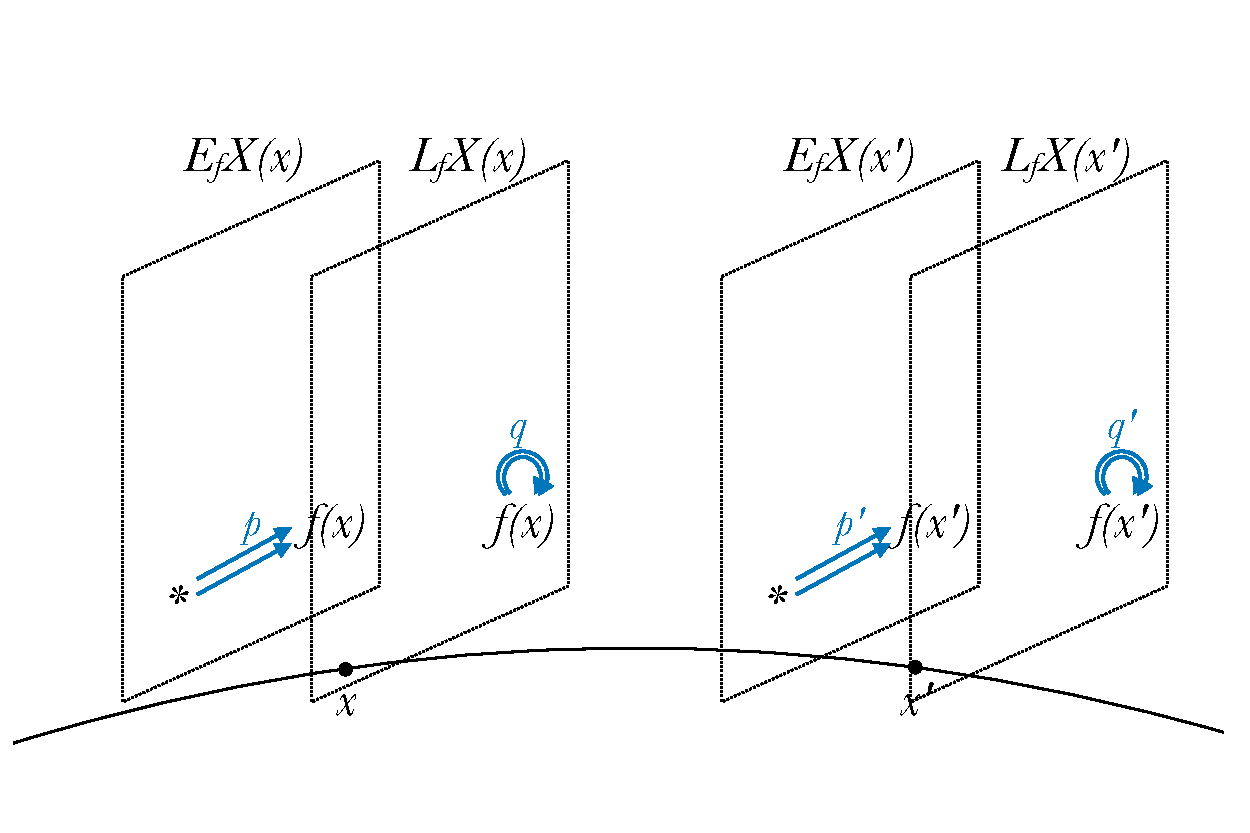
\includegraphics[height=3in,width=4.5in]{torsors_and_gauge}
\caption{Torsors and gauge transformations over $X$. $p$ and $q$ are terms in the fibers of the total spaces $E_fX$ and $L_fX$ respectively. Similarly for $p'$ and $q'$. We can then form $p\cdot q$ and $p'\cdot q'$. If we had a whole section of such $q$ then we could use that to act on the whole of $E_fX$.}
\end{center}
\end{figure}

\mysection{$BG$ classifies bundles, not just equivalence classes}
The classical theorems take the form: taking the pullback of $EG\to BG$ forms a bijection between homotopy classes of maps $f:X\to BG$ and equivalence classes of principal $G$-bundles over $X$. 

\mysection{Universes versus bundles}

\mysection{Eilenberg-Mac Lane spaces}
\emph{Inductive types} are collections of data and rules for mapping out of instances of the collection. For example here is an inductive type defining the natural numbers in Agda:
\begin{code}%
	\>[0]\AgdaKeyword{data}\AgdaSpace{}%
	\AgdaDatatype{nat}\AgdaSpace{}%
	\AgdaSymbol{:}\AgdaSpace{}%
	\AgdaPrimitive{Type}\AgdaSpace{}%
	\AgdaKeyword{where}\<%
	\\
	\>[0][@{}l@{\AgdaIndent{0}}]%
	\>[2]\AgdaInductiveConstructor{zero}\AgdaSpace{}%
	\AgdaSymbol{:}\AgdaSpace{}%
	\AgdaDatatype{nat}\<%
	\\
	%
	\>[2]\AgdaInductiveConstructor{succ}\AgdaSpace{}%
	\AgdaSymbol{:}\AgdaSpace{}%
	\AgdaDatatype{nat}\AgdaSpace{}%
	\AgdaSymbol{$\to$}\AgdaSpace{}%
	\AgdaDatatype{nat}\<%
\end{code}

This theory can be extended to support data having values in the identity types of data that was specified earlier in the definition. Here is the circle defined as a HIT in Cubical Agda:
\begin{code}%
	\>[0]\AgdaKeyword{data}\AgdaSpace{}%
	\AgdaDatatype{circle}\AgdaSpace{}%
	\AgdaSymbol{:}\AgdaSpace{}%
	\AgdaPrimitive{Type}\AgdaSpace{}%
	\AgdaKeyword{where}\<%
	\\
	\>[0][@{}l@{\AgdaIndent{0}}]%
	\>[2]\AgdaInductiveConstructor{point}\AgdaSpace{}%
	\AgdaSymbol{:}\AgdaSpace{}%
	\AgdaDatatype{circle}\<%
	\\
	%
	\>[2]\AgdaInductiveConstructor{loop}\AgdaSpace{}%
	\AgdaSymbol{:}\AgdaSpace{}%
	\AgdaInductiveConstructor{point}\AgdaSpace{}%
	\AgdaOperator{\AgdaFunction{$\equiv$}}\AgdaSpace{}%
	\AgdaInductiveConstructor{point}\<%
\end{code}

Given a group $G$ (meaning, a 0-type) with identity $G.1g$ and multiplication $G.mul$, we can form the Eilenberg-Mac Lane type $K(G, 1)$ as the following HIT:
\begin{code}%
	\>[0]\AgdaKeyword{data}\AgdaSpace{}%
	\AgdaDatatype{eil-mac}\AgdaSpace{}%
	\AgdaSymbol{(}\AgdaBound{G}\AgdaSpace{}%
	\AgdaSymbol{:}\AgdaSpace{}%
	\AgdaFunction{Group}\AgdaSymbol{)}\AgdaSpace{}%
	% \AgdaSymbol{(}\AgdaBound{1g}\AgdaSpace{}%
	% \AgdaSymbol{:}\AgdaSpace{}%
	% \AgdaBound{G}\AgdaSymbol{)}\AgdaSpace{}%
	% \AgdaSymbol{(}\AgdaBound{mult}\AgdaSpace{}%
	% \AgdaSymbol{:}\AgdaSpace{}%
	% \AgdaBound{G}\AgdaSpace{}%
	% \AgdaSymbol{$\to$}\AgdaSpace{}%
	% \AgdaBound{G}\AgdaSpace{}%
	% \AgdaSymbol{$\to$}\AgdaSpace{}%
	% \AgdaBound{G}\AgdaSymbol{)}\AgdaSpace{}%
	\AgdaSymbol{:}\AgdaSpace{}%
	\AgdaPrimitive{Type}\AgdaSpace{}%
	\AgdaKeyword{where}\<%
	\\
	\>[0][@{}l@{\AgdaIndent{0}}]%
	\>[2]\AgdaInductiveConstructor{embase}\AgdaSpace{}%
	\AgdaSymbol{:}\AgdaSpace{}%
	\AgdaDatatype{eil-mac}\<%
	\\
	%
	\>[2]\AgdaInductiveConstructor{emloop}\AgdaSpace{}%
	\AgdaSymbol{:}\AgdaSpace{}%
	\AgdaBound{G}\AgdaSpace{}%
	\AgdaSymbol{$\to$}\AgdaSpace{}%
	\AgdaSymbol{(}\AgdaInductiveConstructor{embase}\AgdaSpace{}%
	\AgdaOperator{\AgdaFunction{$\equiv$}}\AgdaSpace{}%
	\AgdaInductiveConstructor{embase}\AgdaSymbol{)}\<%
	\\
	%
	\>[2]\AgdaInductiveConstructor{emloop-id}\AgdaSpace{}%
	\AgdaSymbol{:}\AgdaSpace{}%
	\AgdaInductiveConstructor{emloop}\AgdaSpace{}%
	\AgdaBound{G.1g}\AgdaSpace{}%
	\AgdaOperator{\AgdaFunction{$\equiv$}}\AgdaSpace{}%
	\AgdaFunction{refl}\AgdaSpace{}%
	\AgdaInductiveConstructor{embase}\<%
	\\
	%
	\>[2]\AgdaInductiveConstructor{emloop-comp}\AgdaSpace{}%
	\AgdaSymbol{:}\AgdaSpace{}%
	\AgdaSymbol{(}\AgdaBound{x}\AgdaSpace{}%
	\AgdaBound{y}\AgdaSpace{}%
	\AgdaSymbol{:}\AgdaSpace{}%
	\AgdaBound{G}\AgdaSymbol{)}\AgdaSpace{}%
	\AgdaSymbol{$\to$}\AgdaSpace{}%
	\AgdaInductiveConstructor{emloop}\AgdaSpace{}%
	\AgdaSymbol{(}\AgdaBound{x}\AgdaSpace{}%
	\AgdaBound{G.mult}\AgdaSpace{}%
	\AgdaBound{y}\AgdaSymbol{)}\AgdaSpace{}%
	\AgdaOperator{\AgdaFunction{$\equiv$}}\AgdaSpace{}%
	\AgdaSymbol{(}\AgdaInductiveConstructor{emloop}\AgdaSpace{}%
	\AgdaBound{x}\AgdaSymbol{)}\AgdaSpace{}%
	\AgdaOperator{\AgdaFunction{∙}}\AgdaSpace{}%
	\AgdaSymbol{(}\AgdaInductiveConstructor{emloop}\AgdaSpace{}%
	\AgdaBound{y}\AgdaSymbol{)}\<%
	\\
	%
	\>[2]\AgdaInductiveConstructor{emsquash}\AgdaSpace{}%
	\AgdaSymbol{:}\AgdaSpace{}%
	\AgdaSymbol{$\forall$}\AgdaSpace{}%
	\AgdaSymbol{(}\AgdaBound{x}\AgdaSpace{}%
	\AgdaBound{y}\AgdaSpace{}%
	\AgdaSymbol{:}\AgdaSpace{}%
	\AgdaDatatype{eil-mac}\AgdaSymbol{)}\AgdaSpace{}%
	\AgdaSymbol{(}\AgdaBound{p}\AgdaSpace{}%
	\AgdaBound{q}\AgdaSpace{}%
	\AgdaSymbol{:}\AgdaSpace{}%
	\AgdaBound{x}\AgdaSpace{}%
	\AgdaOperator{\AgdaFunction{$\equiv$}}\AgdaSpace{}%
	\AgdaBound{y}\AgdaSymbol{)}\AgdaSpace{}%
	\AgdaSymbol{(}\AgdaBound{r}\AgdaSpace{}%
	\AgdaBound{s}\AgdaSpace{}%
	\AgdaSymbol{:}\AgdaSpace{}%
	\AgdaBound{p}\AgdaSpace{}%
	\AgdaOperator{\AgdaFunction{$\equiv$}}\AgdaSpace{}%
	\AgdaBound{q}\AgdaSymbol{)}\AgdaSpace{}%
	\AgdaSymbol{$\to$}\AgdaSpace{}%
	\AgdaBound{r}\AgdaSpace{}%
	\AgdaOperator{\AgdaFunction{$\equiv$}}\AgdaSpace{}%
	\AgdaBound{s}\<%
\end{code}

\mysection{Associated bundles}

\mychapter{Cohomology and characteristic classes}

\mychapter{Connections and Chern-Weil theory}
    
\appendix
\chapter{Appendix}

\bibliography{connections}

\end{document}
